\documentclass[12pt,a4paper]{article}
\usepackage{geometry}

% Page margin layout
\geometry{left=2.3cm,right=2cm,top=2.5cm,bottom=2.0cm}

\usepackage{graphics}
\usepackage{graphicx}
\usepackage{subfigure}
\usepackage{epsfig}
\usepackage{float}
\usepackage{mfirstuc}
\usepackage{hyperref}
\usepackage{amsmath}

\usepackage{booktabs}
\usepackage{threeparttable}
\usepackage{longtable}
\usepackage[ruled,linesnumbered]{algorithm2e}
\usepackage{listings}

% cite package, to clean up citations in the main text. Do not remove.
\usepackage{cite}

\usepackage{color,xcolor}

%% The amssymb package provides various useful mathematical symbols
\usepackage{amssymb}
%% The amsthm package provides extended theorem environments
\usepackage{amsthm}
\usepackage{amsfonts}
\usepackage{enumerate}
\usepackage{enumitem}
\usepackage{listings}

\usepackage{indentfirst}
\setlength{\parindent}{2em} % Make two letter space in the first paragraph
\usepackage{setspace}
\linespread{1.5} % Line spacing setting

\setlength{\parskip}{0.5em} % Paragraph spacing setting

%%%%%%%%%%%%%
\newcommand{\TeamNumber}{2208487}  % Fill your team number here
\newcommand{\Problem}{C}  % Replace your team chosen problem here
\newcommand{\PaperTitle}{To Harvest More: Achieve the Best Trading Strategies on Gold and Bitcoin}  % Change your paper title here
%%%%%%%%%%%%%

\newcommand{\Predictor}{ARIMA }


%% Page header and footer setting
\usepackage{fancyhdr}
\usepackage{lastpage}
\pagestyle{fancy}
\fancyhf{}
\fancyhead[L]{\texttt{Team \#  \TeamNumber }}
\fancyhead[R]{\texttt{Page {\thepage} of \pageref{LastPage}}}



\begin{document}

%%%%%%%%%%%%%%%%%%%%%%%%%%%%%%%%%%%%%%%%%%%%
\makeatletter % change default title style
\renewcommand*\maketitle{%
    \begin{center} 
        \bfseries  % title 
        {\LARGE \@title \par}  % LARGE typesetting
        \vskip 1em  %  margin 1em
        {\global\let\author\@empty}  % no author information
        {\global\let\date\@empty}  % no date
        \thispagestyle{empty}   %  empty page style
    \end{center}%
  \setcounter{footnote}{0}%
}
\makeatother
%%%%%%%%%%%%%%%%%%%%%%%%%%%%%%%%%%%%%%%%%%%%


%%%%%%%%%%%%%%%%%
% Summary sheet
\begin{table}[h]
\renewcommand{\arraystretch}{1.2}
\label{Summary}
\begin{center}
\resizebox{\textwidth}{!}
{\large
\begin{tabular}{c c c c c c c}
{\,} & \textbf{Problem Chosen} & {\qquad \quad} & \textbf{2022} & {\qquad \quad} & \textbf{Team Control Number} & {\,}\\
{} & \raisebox{-2ex}[0cm][0cm]{\LARGE{\textbf{\textcolor{red}{\Problem}}}} & {} & \textbf{MCM/ICM} & {} & \raisebox{-2ex}[0cm][0cm]{\LARGE{\textbf{\textcolor{red}{\TeamNumber}}}} & {}\\
{} & {} & {} & \textbf{Summary Sheet} & {} & {} & {}\\
\bottomrule
\end{tabular}}
\end{center}
\end{table}
\vskip -1.5em
%%


\begin{spacing}{1.2}   % summary line spacing setting


% Enter your summary here replacing the (red) text
% Replace the text from here ...

Traders buy and sell volatile assets to maximize their income. Recently, with the growing interest of the public in cryptocurrencies, gold and bitcoin become a feasible kind of portfolio. But what comes with interest is risk. How can we do our best to increase our income? Our team is requested to determine the trading strategies for a trader which utilizes only the past daily prices. 

As for problem 1, First we plot the price data and found that they show non-stationarity in the sense of mean. We therefore utilize \Predictor to deal with the non-stationarity and predict the future prices of gold and bitcoin. Our choice of parameters is $ARIMA(4,1,4)$ for both bitcoin and gold. Our $ARIMA(4,1,4)$-based predictor shows good capability to accurately predict the price of future.

To find the best timing to sell and buy the two assets, we first rate them with the our well-designed rating system by three important factors:

\begin{itemize}
	\item Changes in value
	\item Moving averages
	\item Bias
\end{itemize}
 

Then from the factors our model further calculates our indicator for risk and trend. By linearly compose these two indicators, we get our main factor, which can give us enough information to make trading decisions.

By utilizing the information we get with our main factor to make trading decisions, we furthermore set thresholds based on our observations and experiments in our data. 

As for problem 2, we dig into the application of Markowiz portfolio theory to our task. By plotting a thermodynamic diagram for various asset allocation schemes, we find that our scheme yields nearly the best result that is possibly for us to get. Moreover, it indicates that we achieve better risk management by maximize the income for taking every unit of risk.

As for problem 3, we test our model by change the commissions for trading bitcoin and gold. By visualizing the result we find that commissions do not have a noteworthy impact on the amount of income of our model, which reveals great stability and scalability for more complicated application. Our model reached a \textbf{annualized return} of $\mathbf{1469.58\%}$, and yielded an \textbf{accumulated equity} of $\mathbf{1.03743 \times 10^6}$ \textbf{USD}. The \textbf{Sharpe ratio} is \textbf{1.1358}, which reveals that our risk-taking strategies perform well compared to a risk-free asset.


\textbf{Key words: ARIMA, Regression, Quantitative Trading, Trading Strategy, Markowiz Portfolio Theory} 

\end{spacing}

\thispagestyle{empty}


%%%%%%%%%%%%%%%%%
\newpage

\title{
\Large{\textcolor{black}{\PaperTitle}}
}




\maketitle



%%%%%%%%%%%%%%%%%
% Table of Contents
\tableofcontents
\setcounter{tocdepth}{2}

%%%%%%%%%%%%%%%%%
\newpage
\setcounter{page}{1}

%% main text

\begin{spacing}{1.2} 



%%%%%%%%%%%%%%%%%
\section{Introduction}
\label{Problem_Statement}

\subsection{Problem Background}
With the popularity of cryptocurrencies and the simplification of trading methods, more of the population become market traders. Some of them expect to outperform inflation, while others want to create wealth. By buying and selling volatile assets frequently, market traders pursue a goal to maximize their total return. Gold and bitcoin enjoy great popularity these days for their complementary characteristics in risk and value. Gold is stable in price and has lower risk while the value of bitcoin varies greatly and thus has a higher risk, as is shown in Figure \ref{figure:prices2in1}.

\begin{figure}[H]
	\centering{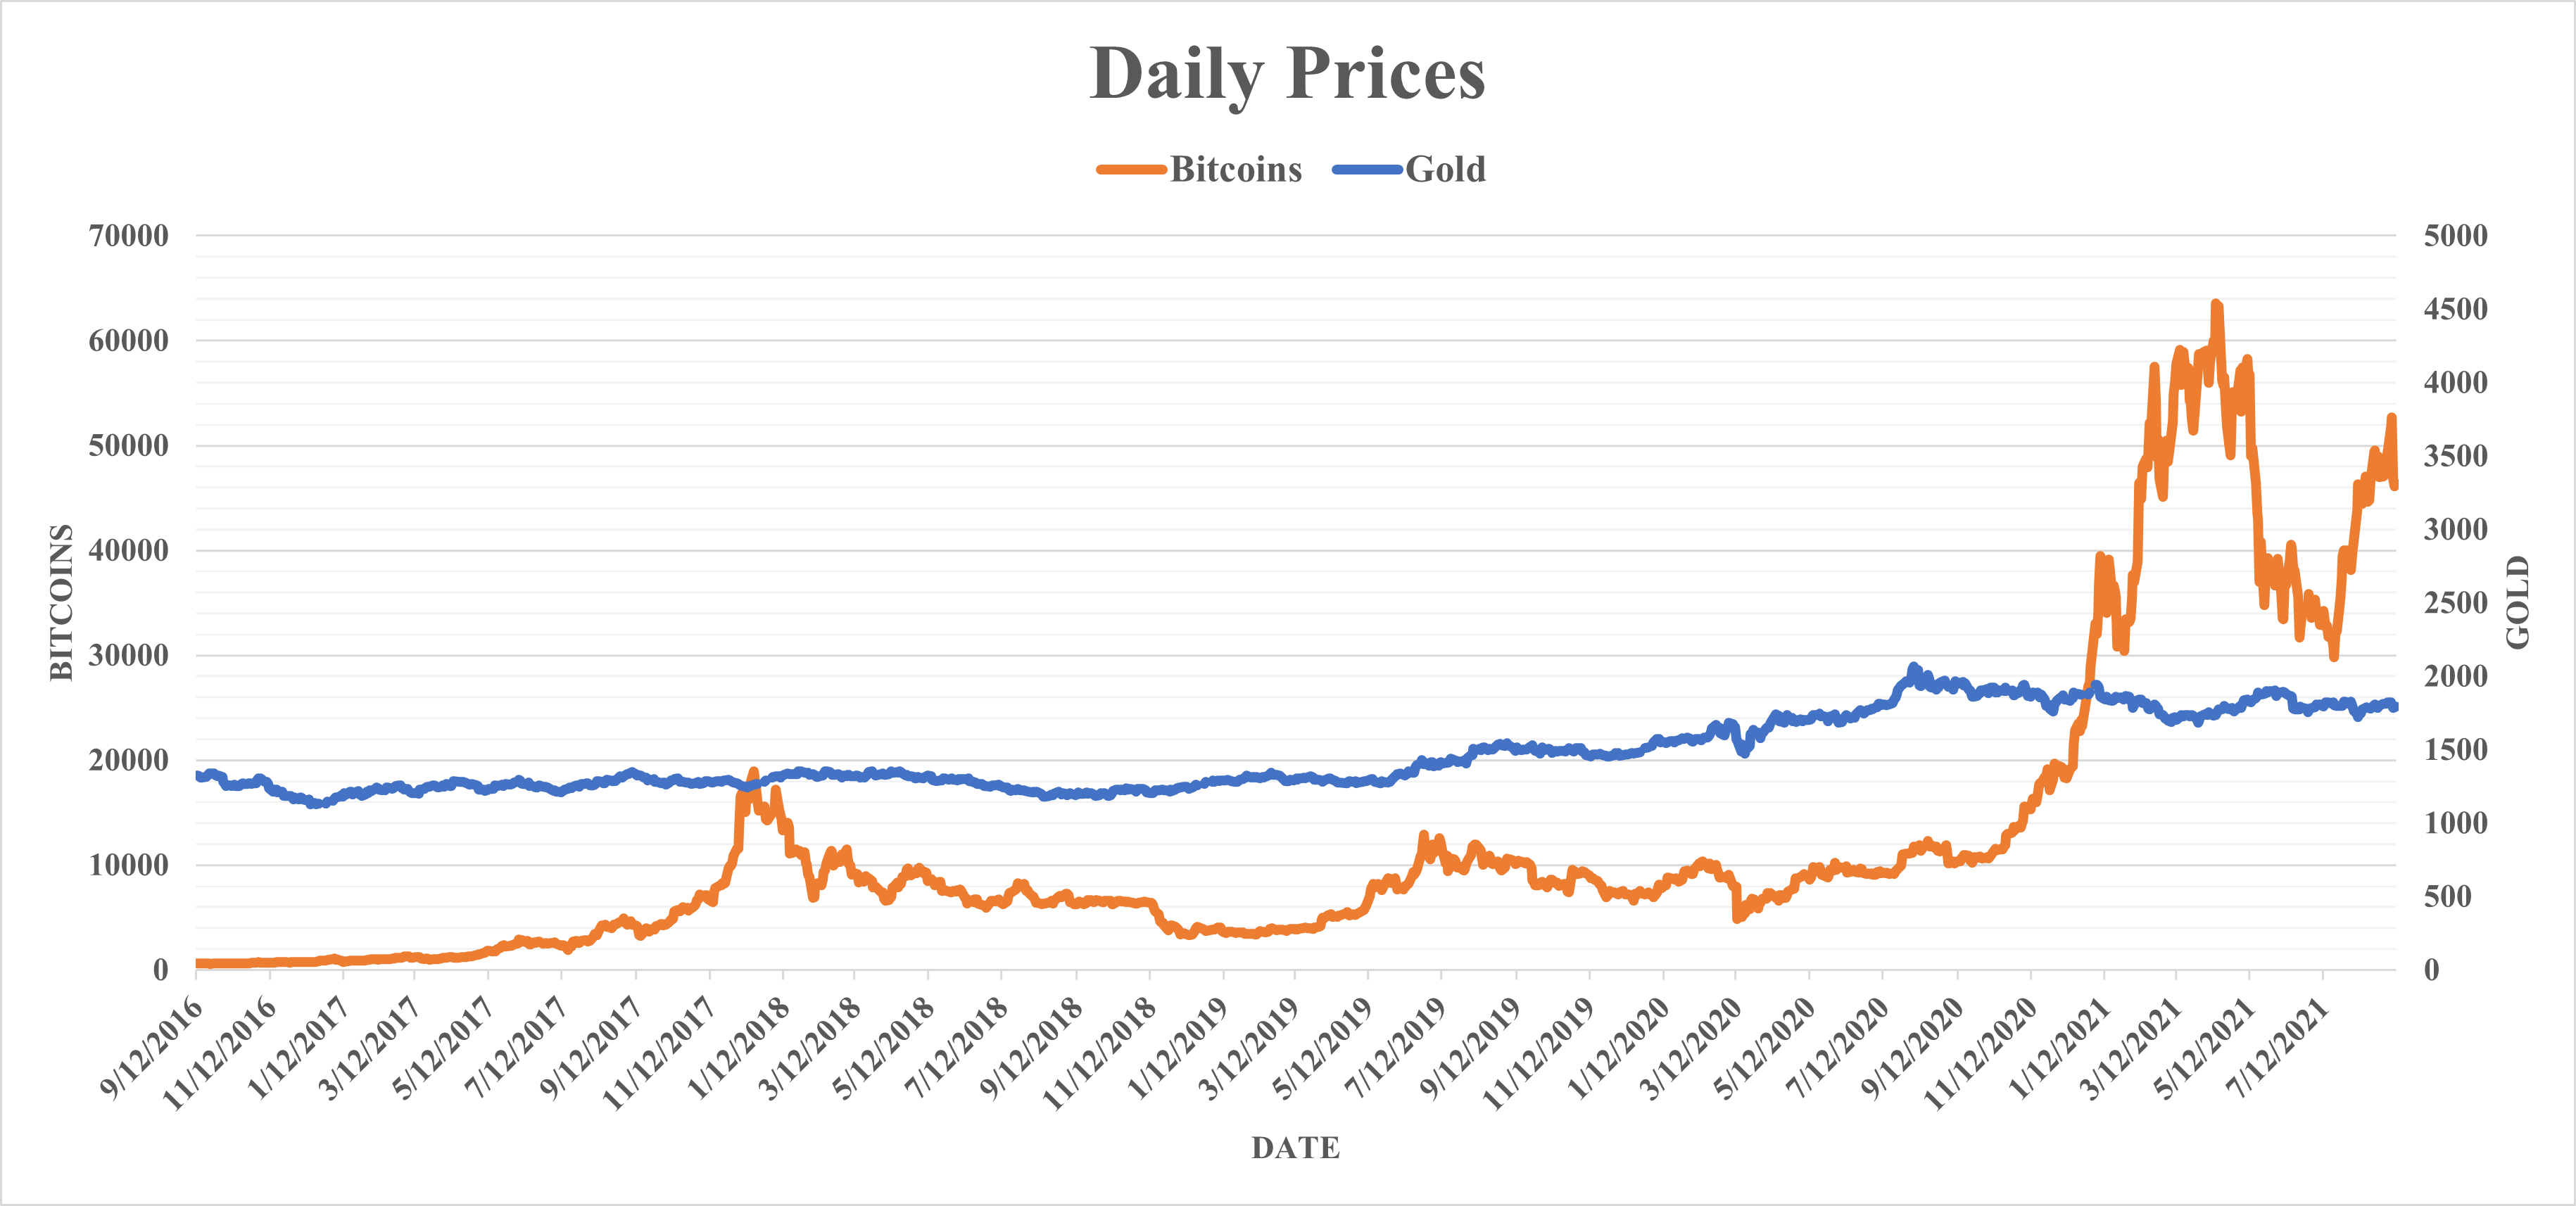
\includegraphics[width=17.0cm]{figures/prices_2in1.png}}
	\caption{Gold and bitcoin daily prices, in U.S. dollars per troy ounce and U.S. dollars per bitcoin. \textbf{Source:} London Bullion Market 
		Association, 9/11/2021 and NASDAQ, 9/11/2021 }
	\label{figure:prices2in1}
\end{figure}

 Regarding trading rules, Gold is only traded on days the market is open while bitcoin are traded every day. Commissions are charged to make each transaction. For market traders to achieve their goals, they need to build a model to determine the strategies to manage their portfolios well.

\subsection{Restatement of the Problem}

\begin{itemize}
	\item Develop a model that gives the best daily trading strategy based only on price data up 
	to that day, and calculate how much the initial \$1000 investment is worth on 9/10/2021 using the 
	model and strategy.
	
	\item Present evidence that this model provides the best strategy.
	
	\item Find how sensitive the strategy is to transaction costs and analyze how the costs
	affect the strategy and results.
	
\end{itemize}

\subsection{Our Approach}

\begin{enumerate}
	\item \textbf{To predict the prices of bitcoin and gold and make decision, we use \textit{\Predictor} (Autoregressive integrated moving average).}
	To predict future prices with existing data is a difficult problem because too many factors may influence the prices. The international situation, national policies, and even social media can have a considerable impact on the prices. Moreover, the data shows non-stationarity. To take as many factors as possible and predict accurately according to their inner laws, we adopt \Predictor to predict the prices, which is proved to give satisfying results.
	
	\item \textbf{To make decision on trading, design a comprehensive rating system to make decisions on trading.} Based on various factor drawn out from price data, we compute our main factor by compose the trend indicator and risk indicator. We then set thresholds based on both our observations and findings in data. Then we decide the final strategies Markowiz portfolio theory.
\end{enumerate}

%%%%%%%%%%%%%%%%%
\section{Assumptions and Justifications}
\label{Assumptions_Justifications}

\subsection{Assumptions}
To simplify the problem stated above, we make following assumptions, each of which is justified properly: 
\begin{enumerate}
	
	\item \textbf{The trader does not have a bias towards a lower risk.} The two given assests, gold and bitcoin, differs a lot in risk. To simplify the problem, we assume that the trader will not prefer lower risk than higher and only cares about higher income.
	
	\item \textbf{The trader will have \$1000 in the beginning, and the transaction commissions for gold and bitcoin are $\alpha_{gold}=1\%$ and $\alpha_{bitcoin}=2\%$, respectively.}

	\item \textbf{The return rate for cash is 0\%} To simplify the problem, we assume that the cash that we hold do not produce any return at all.

	\item \textbf{The market trader sells all of the gold and bitcoin by the end of the five-year trading period, i.e. on 9/10/2021.} Generally, investors cares about funding liquidity. Among cash, gold and bitcoin, only cash can circulate unhindered in the market. So we make this assumption and thus measure the outcome in cash.
	
\end{enumerate}


\subsection{Symbols and Definitions}

\begin{table}[H]
	\renewcommand{\arraystretch}{1.5}
	\caption{Symbols and Definitions.}
	\label{Table_Symbols}
	\begin{center}
		{\footnotesize
			\begin{tabular}{c c}
				\toprule
				{Notations} & {Description} \\
				\midrule
				{$\Delta^ky_t$} & {The k-order difference of the function $y$} \\
				{$PC$}    & {Percentage change} \\ 
				{$P_{0,bitcoin}$}     & { The p-value for ADF test of the raw data of bitcoin} \\ 
				$P_{0,gold}$   & {The p-value for ADF test of the raw data of gold} \\ 
				$P_{1,bitcoin}$     & { The p-value for ADF test of the first-order difference of bitcoin} \\
				$P_{1,gold}$     & {The p-value for ADF test of the first-order difference of gold} \\ 
				$SS$     & {Threshold for main factor to sell certain asset} \\ 
				$BS$    & {Threshold for main factor to buy certain asset} \\ 
				$TI$     & {The trend indicator} \\ 
				$RI$     & {The risk indicator} \\ 
				$MF$     & {The main factor} \\ 
				\bottomrule
		\end{tabular}}
	\end{center}
\end{table}



%%%%%%%%%%%%%%%%%


\section{Data Preprocessing}
\label{DataPreprocessing}


\subsection{Metric Calculating}

\subsubsection{Average Change}

Using the trained predictor, we calculate the average of change in the period of 5,10,15,20,and 25 days.

The change each day is defined as

$$
Percentage \ change = PC = \frac{New \ price-Old \ price}{Old \ price} \times 100\%
$$


The result for the given data is in the \nameref{sec:AppendixFT}. Figure \ref{figure:bitcoin_ac} and Figure \ref{figure:gold_ac} shows the average change we calculated for bitcoin and gold, respectively.


\subsubsection{Bias}

Bias measures how much the closing price shifts from the average price.

The formula to calculate the Bias in a $n$ day period is

$$
Bias = \frac{Closing \ price}{The \ mean \ price \ of \ n \ days} - 1
$$

Bias can help to track the market for the raise and fall of the price, which help us to decide whether and when to sell or buy.

\subsubsection{Moving Averages (MA)}

An $n$ day's MA is the average of the price today and the previous $n-1$ days. Plotting all the MAs in a chart, it can reveal the trend of the price of the given period. Combined with current price, it helps us to find the favorable timing to increase our outcome

\section{Mathematical Modeling}
\label{MathModels}

\subsection{\Predictor Predictor}

\Predictor is widely used for forecasting time series data, which is a generalization of ARMA (autoregressive moving average) model. ARMA requires the mean function of the data to be stationary, because history data of stationary series can be used to predict the future. But time series are not always stationary, so ARIMA take an initial differencing step to eliminate the non-stationarity of the mean function. In this case, we find the first order difference is stationary, so we take first order difference. Figure \ref{figure:flow_chart} shows the procedure we take to build the \Predictor model.

 \begin{figure}[H]
 	\centering{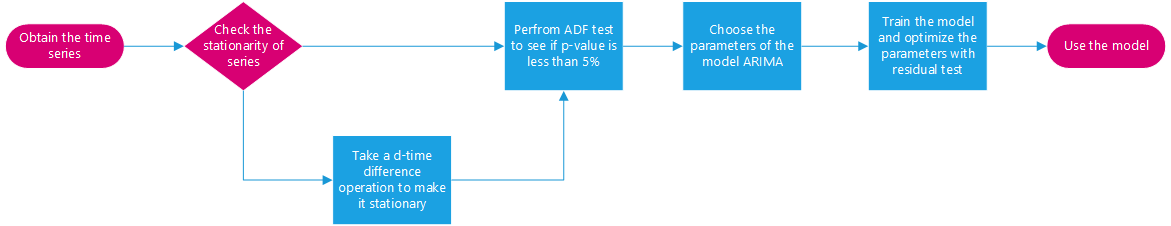
\includegraphics[width=16.0cm]{figures/flow_chart_arima.png}}
 	\caption{Procedure to Build ARIMA Model}
 	\label{figure:flow_chart}
 \end{figure}


To apply the model, we first have to test the stationarity.

\subsubsection{Augmented Dickey-Fuller Test}

An augmented Dickey–Fuller test (ADF) is a kind of hypothesis test. The null hypothesis is 

$$
H_0 \ : \ A \ unit \ root \ is \ present \ in \ a \ time \ series \ sample.
$$

Subject to the $\chi^2$ distribution, we accept it when the observed value of the waviness of the series, $P$, also known as the $p-value$, satisfies

$$
P \ge 0.05
$$

It can test whether the data is stationary or trend-stationary. If the unit root is present in the series, the time-series is non-stationary.

In the raw data, we found

\begin{align*}
	P_{0,bitcoin} &=0.8420802907198858 > 0.05 \\
	P_{0,gold} &=0.9042384812941653 > 0.05 
\end{align*}


So we accept $H_0$. The raw time series is non-stationary.
And in the first-order difference, we found


\begin{align*}
	P_{1,bitcoin}=9.276161468079189e-13 < 0.05 \\
	P_{1,gold}=9.269711421536524e-13 < 0.05
\end{align*}

The first-order difference is stationary, So we plot them in Figure \ref{fig:diff}. 

\begin{figure*}
	\begin{center}
		\subfigure[Gold $1^{st}$ Order Difference]{
			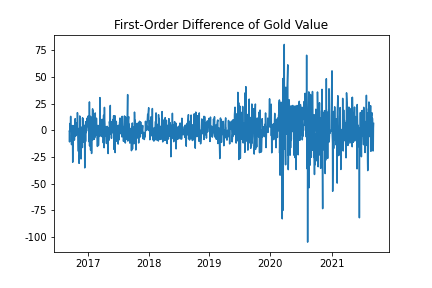
\includegraphics[width=6.0cm]{figures/gold_diff.png}
		}
		\subfigure[Bitcoin $1^{st}$ Order Difference]{
			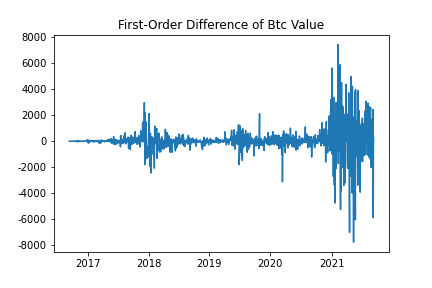
\includegraphics[width=6.0cm]{figures/btc_diff.png}
		}
		\caption{The $1^{st}$ Order Difference}
		\label{fig:diff}
	\end{center}
\end{figure*}

We also can see from the plot that it is stationary. Therefore, we use it for our ARIMA model. The parameter $d$ of $ARIMA(p,d,q)$ is $d=1$.

\subsubsection{Finite Difference}

The difference of a function $y$ is defined as

$$
\Delta^k y_t = \Delta(\Delta^{k-1}y_t)=\Delta^{k-1}y_{t+1}-\Delta^{k-1}y_t=\Sigma_{i=0}^k(-1)^i C_k^iy_{t+k-1} \ (k=1,2,3,\dots)
$$

Specially, the first-order difference, which is commonly used in \Predictor model, is defined as

$$
\Delta y_t = y_{t+1} - y_{t}
$$

Finite difference is useful in processing non-stationary data.

\subsubsection{Choice of Parameters}

To select the best parameters of ARIMA model, we first rely on observation on PACF and ACF plot. And then, if it does not fall in a range that makes sense, we search for possible parameters by grid searching the feasible domain.

\begin{figure*}
	\begin{center}
		\subfigure[Gold ACF Plot]{
			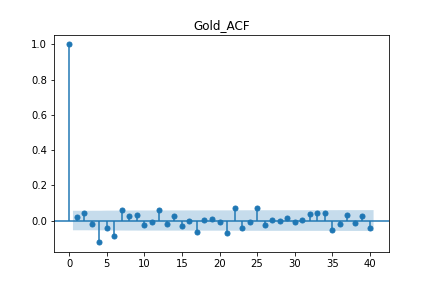
\includegraphics[width=6.0cm]{figures/gold_acf.png}
		}
		\subfigure[Bitcoin ACF Plot]{
			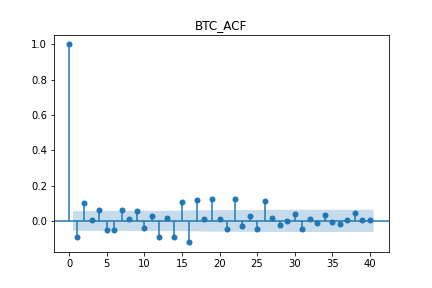
\includegraphics[width=6.0cm]{figures/btc_acf.png}
		}
		\caption{ACF Plot for Gold and Bitcoin}
		\label{fig:acf}
	\end{center}
\end{figure*}

The parameter $p$ of ARIMA(p,d,q) is the number of lag observations in the model, which is also known as the lag order. To assign $p$, ACF plot in Figure \ref{fig:acf} is inspected. We find that $p=4$ is the best choice for both bitcoin and gold.

\begin{figure*}
	\begin{center}
		\subfigure[Gold PACF Plot]{
			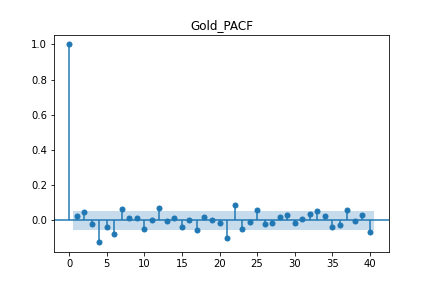
\includegraphics[width=6.0cm]{figures/gold_pacf.png}
		}
		\subfigure[Bitcoin PACF Plot]{
			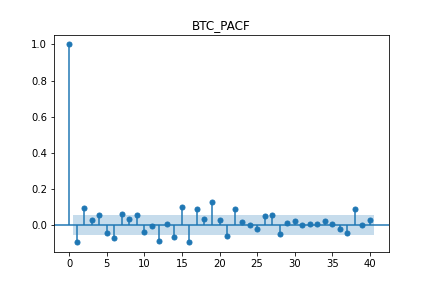
\includegraphics[width=6.0cm]{figures/btc_pacf.png}
		}
		\label{fig:pacf}
		\caption{PACF Plot for Gold and Bitcoin}
	\end{center}
\end{figure*}

The parameter $q$ is the size of moving average window, which is also called the order of moving window. To assign $q$, PACF plot in Figure \ref{fig:pacf} is inspected. We find that $q=4$ is the best choice for both bitcoin and gold.


\subsubsection{Residual Test and Durbin-Watson Test}
To test whether our model has extracted all information in the data, we inspect the residuals and test if they look like white noise. White noise residuals reveal that all information to predict has been extracted, so that we can utilize them to predict the future. And what is left is only random perturbation and is of no use for our \Predictor predictor. To carry out the test, we first plot the residual Q-Q plot and then carry our a Durbin-Watson(DW) test. The test results are as follows.

\begin{enumerate}
	\item \textbf{Residual Q-Q Plot}
	A Quantile-Quantile plot (Q-Q plot) shows the "match" of an observed distribution with a theoretical distribution, almost always the normal distribution. We plot the Q-Q plot and find that the residual distribution is roughly the same as the normal distribution, or is similar to white noise.
	
	\begin{figure}
		\begin{center}
			\subfigure[Gold Residual Q-Q Plot]{
				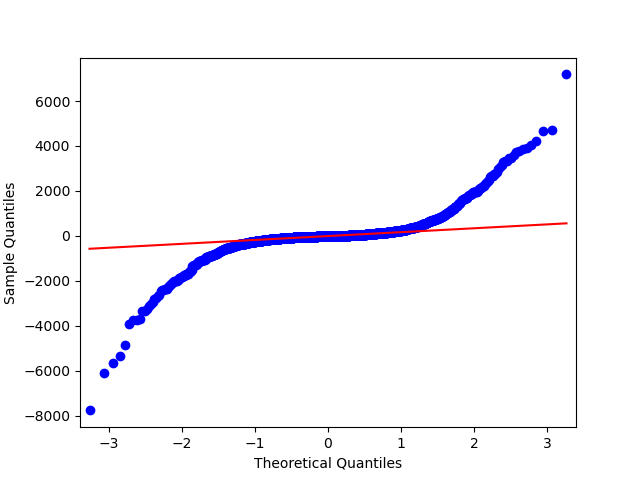
\includegraphics[width=6.0cm]{figures/btc_arima_residual.png}
			}
			\subfigure[Bitcoin Residual Q-Q Plot]{
				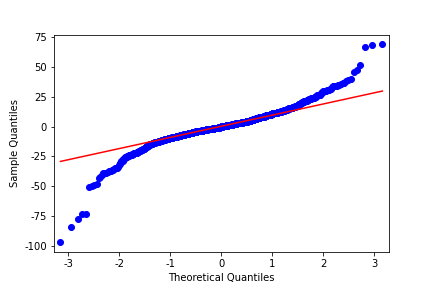
\includegraphics[width=6.0cm]{figures/gold_arima_residule.png}
			}
		\end{center}
			\caption{Residual Q-Q Plot for Gold and Bitcoin}
		\label{fig:qq_plot}
	\end{figure}

	We can see in Figure \ref{fig:qq_plot} that the scatters appears to be around a straight line, which indicates our parameters are good enough to predict the future.
	
	\item \textbf{DW Test}
	DW test is commonly used for test whether autocorrelation presents in the residuals from a regression analysis. The DW statistics has a null hypothesis
	
$$
	H_0 \ : \ \rho = 0	
$$
	And the test statistic is
	
	\begin{equation}\label{eqn:d}
		d \ = \ \frac{\Sigma_{t=2}^T(e_t-e_{t-1})^2}{\Sigma_{t=1}^T e_t^2}
	\end{equation}

	We calculate $d$ in equation \ref{eqn:d}, which is the approximation of $2(1-\hat{\rho})$, where $\hat{\rho}$ is the sample autocorrelation of the residuals. So $d=2$ indicates no autocorrelation. In our case, we calculate the values in by equation \ref{eqn:d}, and find
	$$
	d \ = \ 2.0179203733750732
	$$
	which is very close to 2, indicating very low autocorrelation. 
\end{enumerate}

\subsection{Trade Decision}

\subsubsection{Position Management}
\label{sec:pos_management}

According to Markowitz portfolio theory, the final return of using a multi-asset portfolio investment can reach the weighted average of each asset's return, but the portfolio can significantly reduce systematic risk. The aim is to flatten the return curve and reduce retracements.

Markowitz utilizes mean-variance analysis in his model to measure the expected return and risk of each asset, and in the following, we will also use this model to quantify the expected return and risk of this portfolio of bitcoin and gold.

To measure the risk of the portfolio, we calculate the standard deviation. The standard deviation of the portfolio is defined as

$$
	\sigma = \sqrt{\mathbf{w_T}  \cdot \Sigma \cdot \mathbf{w}}
$$

Where $\sigma$ is the standard deviation of the portfolio, $\Sigma$ is the covariance matrix of the portfolio, and vector $\mathbf{w}$ is the weight of the portfolio. So to solve the given problem, the vector $\mathbf{w}$ is defined as 

$$
\mathbf{w} \ = \ (w_{cash},w_{bitcoin},w_{gold})
$$

Where $w_{cash}$, $w_{bitcoin}$, and $w_{gold}$ is the weight in the portfolio for cash, bitcoin and gold, respectively. 

To measure the return of the portfolio, we use the annualized return of the portfolio.

\begin{figure}[H]
	\centering{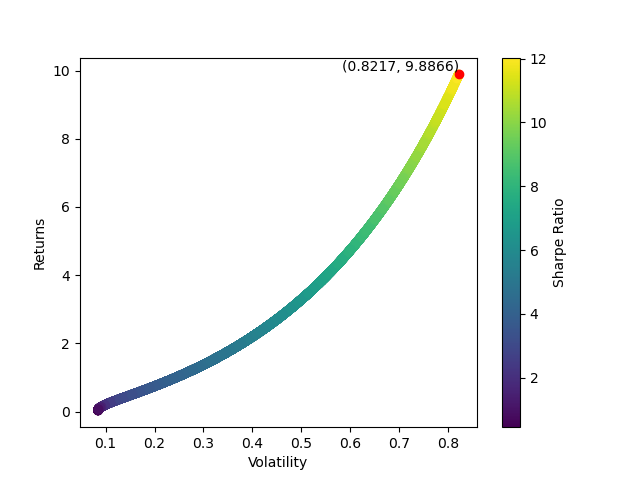
\includegraphics[width=8.0cm]{figures/markowiz_sim.png}}
	\caption{Application of Markowiz Theory}
	\label{figure:markowiz}
\end{figure}

Using the mean-variance analysis, we try to find a portfolio that minimize the risk and maximize the return. In our model, we use the Monte-Carlo method to simulate the positions of bitcoin and gold. The result of the simulation is plotted in Figure \ref{figure:markowiz}.
We can conclude from the figure that if the trader is looking for a higher Sharpe Ratio, we should look for the point with the largest value of the vertical coordinate over the horizontal coordinate, or on the top-left area of the figure.
Extracting the portfolio data behind this point, we find that most portfolios with a Sharpe Ratio of 10 or higher have a portfolio share of 95\% or more in bitcoin.
Therefore, we conclude to invest bitcoin as much as possible in the whole portfolio. When both gold and bitcoin are on an upward trend, traders are supposed to buy more bitcoin for their portfolio to achieve a high expected return.


\subsubsection{Rating Gold and Bitcoin}

Based on the closing price every day, we first calculates the required normalized factors using including the change today, and the average change of 15 days and the bias, for both bitcoin and gold. Then our model predict the price the next day with ARIMA model.

Then, we calculate the indicators with the formula below for bitcoin and gold. 


\begin{align*}
	Trend \ indicator &= TI = 0.7 \times 30 \ day's \ average change \ + \ 0.3 \times 20 \ day's \ average \ bias \\
	Risk \ indicator &= RI = 0.4 \times Normalized \ 15 \ day's \ average \ change + 0.6 \times bias
\end{align*}

Then we compose $TI$ and $RI$ linearly with ratios chosen according to Markowiz portfolio theory and then normalize it to get our main factor ($MF$) for bitcoin and gold. 

We set following thresholds for selling or buying bitcoin and gold in Table \ref{table:threshold}.

\begin{table}[H]
	\renewcommand{\arraystretch}{1.5}
	\caption{Trading Thresholds.}
	\label{table:threshold}
	\begin{center}
		{\footnotesize
			\begin{tabular}{c c c}
				\toprule
				{ } & {Bitcoin} & {Gold} \\
				\midrule
				Buy($BS$) & 0.775 & 0.57 \\
				Sell($SS$) & 0.55 & 0.3 \\
				\bottomrule
		\end{tabular}}
	\end{center}	
\end{table}

Then, we trade bitcoin and gold subject to the following rules.

\begin{center}
	\begin{tabular}{ |c|c|c|c| } 
		\hline
		& $MF_{bitcoin} > BS_{bitcoin}$ & $Others$ & $MF_{bitcoin} < SS_{bitcoin}$ \\ 
		\hline
		$MF_{gold} > BS_{gold}$ & \textbf{\textit{Further Judgment Required}}  & Buy gold & Sell bitcoin and buy gold  \\ 
		\hline
		Others & Buy bitcoin & Do nothing & Sell bitcoin \\
		\hline
		$MF_{gold} < SS_{gold}$ & Sell gold and buy bitcoin & Sell gold & Sell both \\ 
		\hline
	\end{tabular}
\end{center}

When further judgment is required, we come up with the following factor $F$ 

$$
F=2.5 \times (MF_{bitcoin}-BS_{bitcoin})-(MF_{gold}-BS_{gold})
$$

Then, our model recommend buying gold when $F<0$ and buying bitcoin when $F>0$. In the above formula, the ratio $2.5$ comes from the weights that reach the maximum in return that we find in the previous sub-section \nameref{sec:pos_management}.

%%%%%%%%%%%%%%%%%
\section{Results and Solutions}
\label{Results_Solutions}

\begin{figure}[H]
	\centering{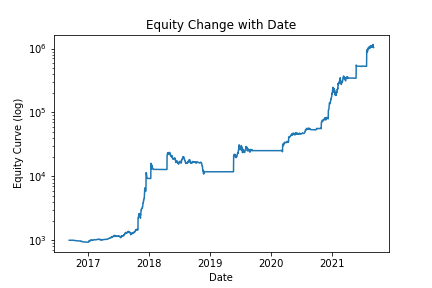
\includegraphics[width=8.0cm]{figures/equity_change.png}}
	\caption{Equity Change Result}
	\label{figure:equity_change}
\end{figure}

As is plotted in Figure \ref{figure:equity_change}, our equity change rises a lot with time going by. From the plot we can know the following facts.

\begin{itemize}
	\item \textbf{Our strategies work well to maximize income.} As is seen in the plot, the equity rises in the order of magnitude from $10^3$ to $10^6$, which is a considerable achievement.
	
	\item \textbf{Our strategies has a distinct feature that it has very low retracement.} As is seen in the plot, only there are only a few retracements, all of which have small value changes. It reveals that we have a good performance in dealing with risks.
\end{itemize}

The detailed performance data is shown in Table \ref{table:performance}. From the table we can have a quantitative view on the brilliant performance of our model.

\begin{table}[H]
	\renewcommand{\arraystretch}{1.5}
	\caption{Performance Data}
	\label{table:performance}
	\begin{center}
		{\footnotesize
			\begin{tabular}{c c }
				\toprule
				Performance Indicator & Measurement\\
				\midrule
				Accumulated Equity & $1.03743 \times 10^6$ \\
				Annualized Return & 1469.58\% \\
				Maximum Retracement & -53.90\% \\
				Annualized Return/Retracement Ratio & 27.77 \\
				Sharpe Ratio & 1.1358 \\
				\bottomrule
		\end{tabular}}
	\end{center}	
\end{table}



%%%%%%%%%%%%%%%%%
\section{Sensitivity Analysis}
\label{SensitivityAnalysis}

For each transaction, a commission is charged. The commission can also have an impact on our model. We tested our model with different commissions and found that the level of commission does not significantly affect our model.

 \begin{figure}[H]
	\centering{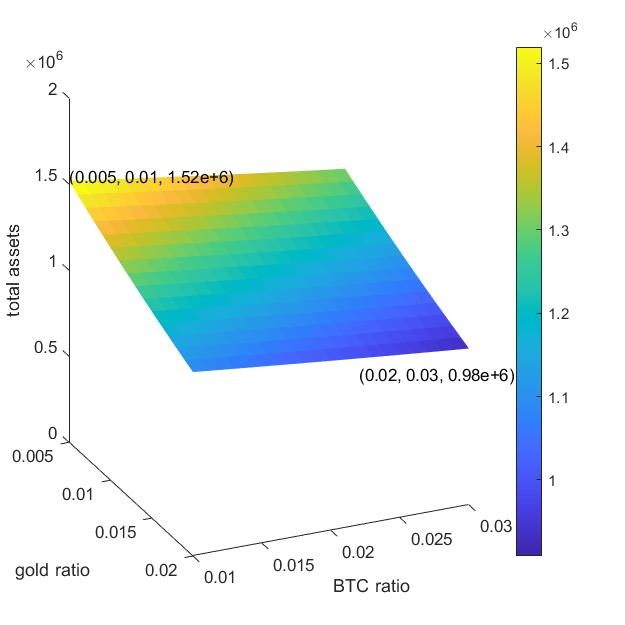
\includegraphics[width=8.0cm]{figures/sensitive_test.jpg}}
	\caption{Equity Change with Commissions}
	\label{figure:sensitive_test}
\end{figure}

By changing commissions and recalculating the total assets we get, we plot Figure \ref{figure:sensitive_test}, from which we can draw the following conclusions

\begin{enumerate}
	\item Commissions may influence the equity change in the end, but the range is considered small, which reveals great stability of our model.
	
	\item From the figure we plot, we find that commissions for bitcoin have a stronger impact on the income. It is because to reach higher income, we hold more bitcoin so that when commissions go higher, we are charged much more.
	
	\item The given commissions is higher than the commissions in the real world, 0.02\% for bitcoin and 0.05\% for gold. When choosing the thresholds for trading, we can choose more suitable parameters and trade in lower frequencies to reduce frictional costs.
\end{enumerate}

%%%%%%%%%%%%%%%%%
\section{Strength and Weakness}
\label{Strength_Weakness}


\subsection{Strength}

The models have the following strengths:

\begin{itemize}
\item \textbf{Our model yields considerable income}

\item \textbf{Our model do not involve artificial neural network, which saves computational resources and improves interpretability.}

\item \textbf{Our model build up a fair system to assess a financial asset.}

\item \textbf{Our model can be generalized to all problems in trading.}

\end{itemize}


\subsection{Weakness}

Though our model performs well, the models have following weaknesses:

\begin{itemize}
\item \textbf{We do not consider factors other than prices.}

\item \textbf{The choice of our model's parameters relies on experience and grid search.}
\end{itemize}


%%%%%%%%%%%%%%%%%
\section{Conclusions}
\label{Conclusions}

In this paper, we build a \Predictor based predictor and the rating-based decision maker to enhance the income of trading gold, and bitcoin. First, we preprocess the data and calculate various factors. Then, we do feature engineering by finite difference to deal with non-stationarity. After that, we use a ARIMA(4,1,4) predictor to predict the price in the future. Finally, we design a rating system and then derive our main factor to decide whether to buy, hold, or sell bitcoin and gold, and our strategies is test with Markowiz portfolio theory. Sensitive tests  are carried out to find that our model will remain stable when commissions change. We measured our model by performance indicators like annualized return, retracement, and Sharpe ratio. Our model yields satisfying results.




%%%%%%%%%%%%%%%%%
\newpage
\begin{thebibliography}{00}

%% \bibitem{label}
%% Text of bibliographic item

\bibitem{Du2021}
Lin Hongmei,Du Jinyan,Zhang Shaodong. Sharpe ratio: estimation method, applicability and empirical analysis[J]. Journal of Statistics,2021,2(06):73-88.DOI:10.19820/j.cnki.issn2096-7411.2021.06.006.

\bibitem{Sun2020}
Sun, Lipo. An empirical study of Makowitz's portfolio theory based on Python[J]. Times Finance,2020(25):46-47+50.

\bibitem{Pierre2020}
Pierre Rostan,Alexandra Rostan,Mohammad Nurunnabi. Options trading strategy based on ARIMA forecasting[J]. PSU Research Review,2020.


\bibitem{Marcos2018}
Marcos Lopez dai Prado, \textit{Advances in Financial Machine} Learning[M]:75-82. ISBN 978-1119482086

\bibitem{Li2017}
Li F. Modelling the stock market using a multi-scale approach[D]. University of Leicester, 2017.

\bibitem{Lin2016}
Lin Xiaoming, A preliminary exploration of Huatai's multi-factor model system [R], Huatai Securities, 2016.

\bibitem{Pang2005}
Marling H, Emanuelsson S. The Markowitz Portfolio Theory[J]. November, 2012, 25: 2012.


\end{thebibliography}
\addcontentsline{toc}{section}{References}


\addtocounter{page}{-1}
\thispagestyle{empty}

%%%%%%%%%%%%%%%%%
\newpage
\addtocounter{page}{-1}
\thispagestyle{empty}

{\centering\section*{Memorandum to the Trader}}

Considering the intensely changing financial markets and the difficulty of handling your portfolio, using an appropriate model to make predictions and strategies to trade are of vital importance to improve income. It is a great honor for us to develop the model for you to buy, hold and sell your assets. Here is our model based on \textbf{\Predictor} and strategies for you to trade your assets effectively.  
	
\begin{enumerate}
	\item Our model calculates the required normalized factors using the closing price every day,including the change today, the average change of 15 days and the bias, for both bitcoin and gold. Then our model predict the price the next day with ARIMA model.
	 
	\item Based on the calculated values and our research, we calculate the indicators with the formula below for bitcoin and gold. 
	

\begin{align*}
	Trend \ indicator &= TI = 0.7 \times 30 \ day's \ average change \ + \ 0.3 \times 20 \ day's \ average \ bias \\
	Risk \ indicator &= RI = 0.4 \times Normalized \ 15 \ day's \ average \ change + 0.6 \times bias
\end{align*}
	
	Then we compose $TI$ and $RI$ linearly with ratios chosen according to Markowiz's asset portfolio model and then normalize it to get our main factor ($MF$) for bitcoin and gold. 
	
	\item We set following thresholds for selling or buying bitcoin and gold in Table \ref{table:memo_threshold}.
	
	\begin{table}[H]
		\renewcommand{\arraystretch}{1.5}
		\caption{Trading Thresholds.}
		\label{table:memo_threshold}
		\begin{center}
			{\footnotesize
				\begin{tabular}{c c c}
					\toprule
					{ } & {Bitcoin} & {Gold} \\
					\midrule
					Buy($BS$) & 0.775 & 0.57 \\
					Sell($SS$) & 0.55 & 0.3 \\
					\bottomrule
			\end{tabular}}
		\end{center}	
	\end{table}

	Our model trades bitcoin and gold subject to the following rules.
	
	\begin{center}
		\begin{tabular}{ |c|c|c|c| } 
			\hline
			 & $MF_{bitcoin} > BS_{bitcoin}$ & $Others$ & $MF_{bitcoin} < SS_{bitcoin}$ \\ 
			\hline
			$MF_{gold} > BS_{gold}$ & \textbf{\textit{Further Judgment Required}}  & Buy gold & Sell bitcoin and buy gold  \\ 
			\hline
			Others & Buy bitcoin & Do nothing & Sell bitcoin \\
			\hline
			$MF_{gold} < SS_{gold}$ & Sell gold and buy bitcoin & Sell gold & Sell both \\ 
			\hline
		\end{tabular}
	\end{center}

	When further judgment is required, we come up with the following factor $F$ 
	
	$$
	F=2.5 \times (MF_{bitcoin}-BS_{bitcoin})-(MF_{gold}-BS_{gold})
	$$
	
	Then, our model recommend buying gold when $F<0$ and buying bitcoin when $F>0$.
\end{enumerate}

With above strategies, our model achieve great income. The performance of our model is as follows

	\begin{table}[H]
	\renewcommand{\arraystretch}{1.5}
	\caption{Performance}
	\label{table:memo_performance}
	\begin{center}
		{\footnotesize
			\begin{tabular}{c c }
				\toprule
				Performance Indicator & Measurement\\
				\midrule
				Accumulated Equity & $1.03743 \times 10^6$ \\
				Annualized Return & 1469.58\% \\
				Maximum Retracement & -53.90\% \\
				Annualized Return/Retracement Ratio & 27.77 \\
				Sharpe Ratio & 1.1358 \\
				\bottomrule
		\end{tabular}}
	\end{center}	
\end{table}


We appreciate this opportunity to help you to build up a trading strategy for cash, gold and bitcoin, and we firmly believe that our model can be utilized in your tradings to maximize your income. Feel free to contact us for further information on the proposal.

Sincerely yours

\textit{MCM 2022 Team}



\end{spacing}


%%%%%%%%%%%%%%%%%
\newpage
%% The Appendices part is started with the command \appendix;
%% appendix sections are then done as normal sections
\appendix
\addtocounter{page}{-1}
\thispagestyle{empty}

\section*{Appendix: Figures and Tables}
\label{sec:AppendixFT}

\begin{figure}[H]
	\centering{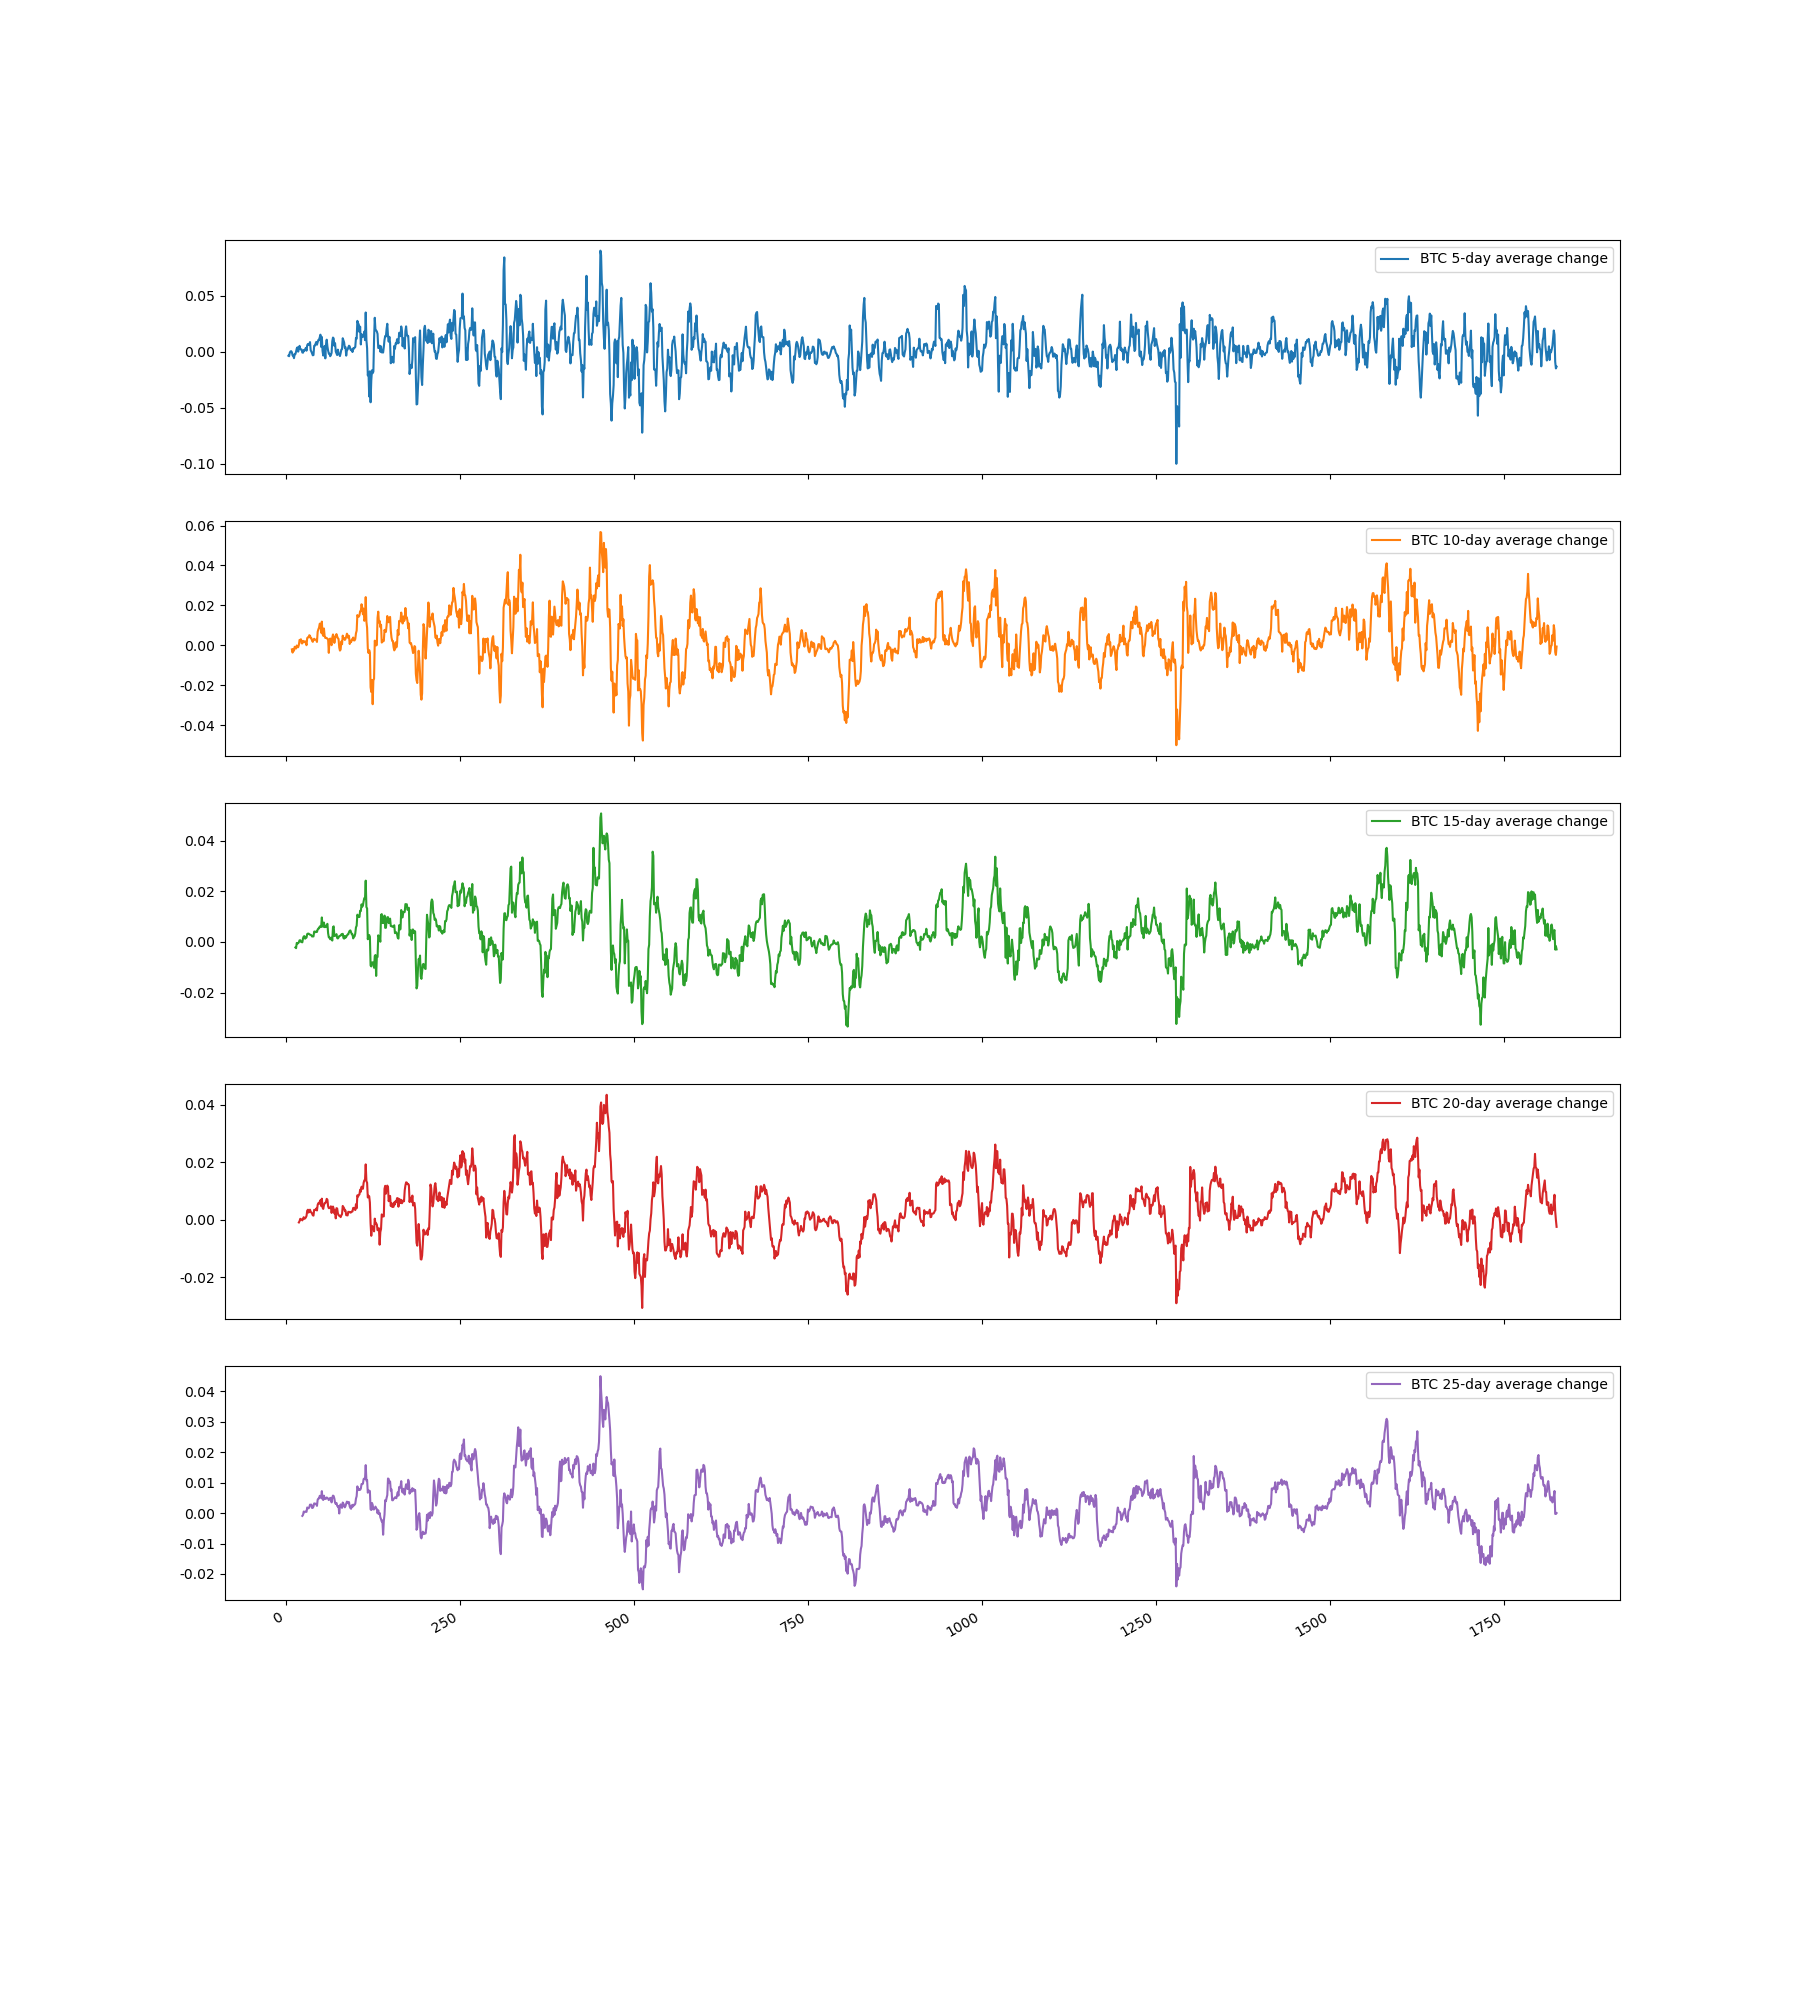
\includegraphics[width=17.0cm]{figures/bitcoin_ac.png}}
	\caption{ Average Change in 5,10,15,20,25 days for bitcoin}
	\label{figure:bitcoin_ac}
\end{figure}

\begin{figure}[H]
	\centering{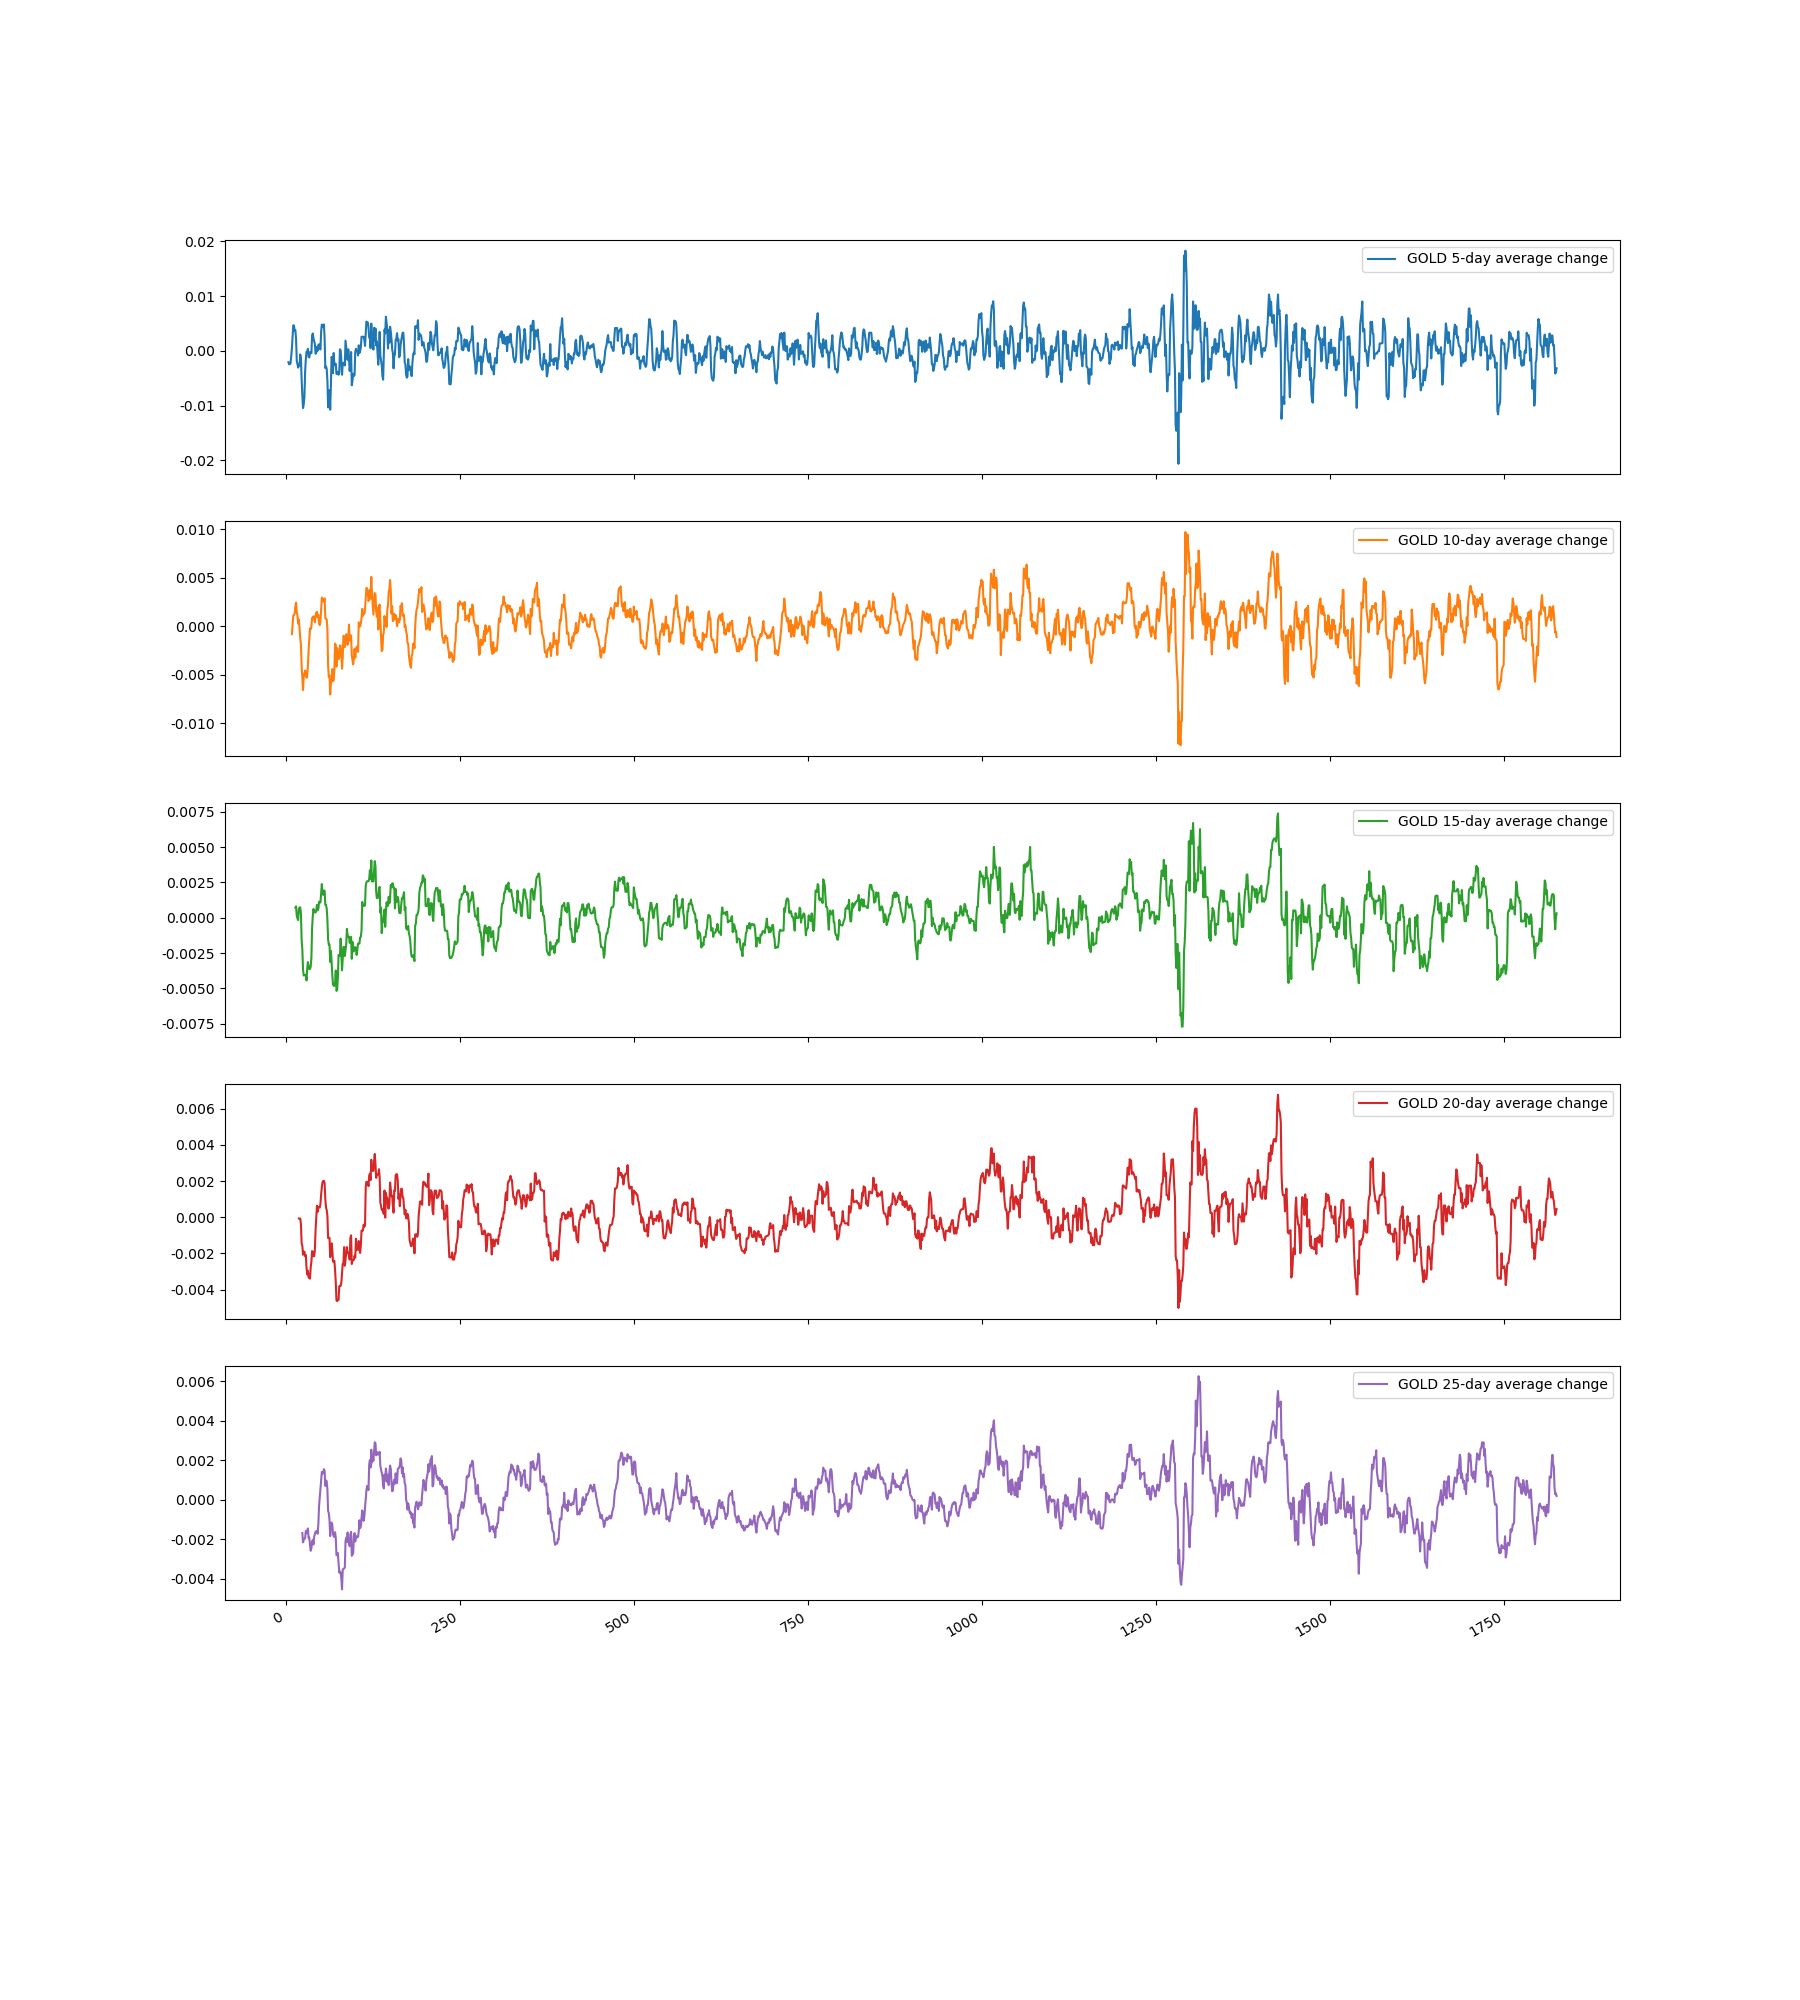
\includegraphics[width=17.0cm]{figures/gold_ac.png}}
	\caption{ Average Change in 5,10,15,20,25 days for gold }
	\label{figure:gold_ac}
\end{figure}


\end{document}


%% End of template
